%%%%%%%%%%%%%%%%%%%%%%%%%%%%%%%%%%%%%%%%%%%%%%%%%%%%%%%%%%%%%%%%%%%%%%%%%%%%%%%%
% TUM-Vorlage: Präsentation
%%%%%%%%%%%%%%%%%%%%%%%%%%%%%%%%%%%%%%%%%%%%%%%%%%%%%%%%%%%%%%%%%%%%%%%%%%%%%%%%
%
% Rechteinhaber:
%     Technische Universität München
%     https://www.tum.de
% 
% Gestaltung:
%     ediundsepp Gestaltungsgesellschaft, München
%     http://www.ediundsepp.de
% 
% Technische Umsetzung:
%     eWorks GmbH, Frankfurt am Main
%     http://www.eworks.de
%
%%%%%%%%%%%%%%%%%%%%%%%%%%%%%%%%%%%%%%%%%%%%%%%%%%%%%%%%%%%%%%%%%%%%%%%%%%%%%%%%

%%%%%%%%%%%%%%%%%%%%%%%%%%%%%%%%%%%%%%%%%%%%%%%%%%%%%%%%%%%%%%%%%%%%%%%%%%%%%%%%
% \PassOptionsToPackage{draft}{graphicx}
\documentclass[utf8, 8pt, t]{beamer}

\usepackage{soul}

%\usepackage[utf8]{inputenc} % Textkodierung: UTF-8
\usepackage[T1]{fontenc} % Zeichensatzkodierung

\usepackage{calc} % Berechnungen

\usepackage[ngerman]{babel} % Deutsche Lokalisierung
\usepackage{graphicx} % Grafiken
\usepackage[absolute, overlay]{textpos} % Positionierung

% Silbentrennung:
\usepackage{hyphenat}
%\tolerance 2414
%\hbadness 2414
%\emergencystretch 1.5em
%\hfuzz 0.3pt
%\widowpenalty=10000     % Hurenkinder
%\clubpenalty=10000      % Schusterjungen
%\vfuzz \hfuzz

% Euro-Symbol:
\usepackage[gen]{eurosym}
\DeclareUnicodeCharacter{20AC}{\euro{}}

% Schriftart Helvetica:
\usepackage[scaled]{helvet}
\renewcommand{\familydefault}{\sfdefault}

\usepackage{mathptmx} % skalierbare Formelschriften

\usepackage{tabularx}

\usepackage{multicol} % mehrspaltiger Text

\usepackage{tikz}
\usetikzlibrary{arrows, shapes, shapes.multipart, trees, positioning,
    backgrounds, fit, matrix}
\usepackage{forest}

% Diagramme:
\usepackage{pgfplots}
\pgfplotsset{compat=default}

% Erweiterbare Fusszeile:
\newcommand{\PraesentationFusszeileZusatz}{}

\usetikzlibrary{fit}
\usepackage{verbatim}
\usepackage{listings}
\usepackage{moeptikz}
 % !!! NICHT ENTFERNEN !!!
%%%%%%%%%%%%%%%%%%%%%%%%%%%%%%%%%%%%%%%%%%%%%%%%%%%%%%%%%%%%%%%%%%%%%%%%%%%%%%%%
% TUM-Vorlage: Personenspezifische Informationen
%%%%%%%%%%%%%%%%%%%%%%%%%%%%%%%%%%%%%%%%%%%%%%%%%%%%%%%%%%%%%%%%%%%%%%%%%%%%%%%%
%
% Rechteinhaber:
%     Technische Universität München
%     https://www.tum.de
% 
% Gestaltung:
%     ediundsepp Gestaltungsgesellschaft, München
%     http://www.ediundsepp.de
% 
% Technische Umsetzung:
%     eWorks GmbH, Frankfurt am Main
%     http://www.eworks.de
%
%%%%%%%%%%%%%%%%%%%%%%%%%%%%%%%%%%%%%%%%%%%%%%%%%%%%%%%%%%%%%%%%%%%%%%%%%%%%%%%%

% Für die Person anpassen:

\newcommand{\PersonTitel}{}
\newcommand{\PersonVorname}{}
\newcommand{\PersonNachname}{}
\newcommand{\PersonFunktion}{}
\newcommand{\PersonStadt}{Garching b. München}
\newcommand{\PersonAdresse}{%
    Boltzmannstr.~3\\%
    85748~\PersonStadt%
}
\newcommand{\PersonTelefon}{}
\newcommand{\PersonFax}{+49}
\newcommand{\PersonEmail}{htum.de}
\newcommand{\PersonWebseite}{win.tum.de}

\newcommand{\LehrstuhlName}{Chair of Network Architectures and Services}



\hyphenation{} % eigene Silbentrennung
                    % !!! DATEI ANPASSEN !!!
%%%%%%%%%%%%%%%%%%%%%%%%%%%%%%%%%%%%%%%%%%%%%%%%%%%%%%%%%%%%%%%%%%%%%%%%%%%%%%%%
\usepackage{soul}
\renewcommand{\PersonTitel}{}
\newcommand{\Datum}{\today}

\renewcommand{\PraesentationFusszeileZusatz}{TMA'17 RIPE Atlas Lab}

\title{TMA 2017 PhD School --- RIPE Atlas Lab}
\author{Emile Aben (RIPE NCC), Quirin Scheitle(TUM)}
\institute[]{\UniversitaetName \\ \FakultaetName}
\date[\Datum]{Dublin, June 20, 2017}
\subject{}
% Fix terminology
\usepackage{tikz}

\colorlet{tablelight}{black!15}
\colorlet{tabledark}{black!40}

\usepackage{xspace}
%\usepackage{todonotes}
\usepackage{tikz}
\usepackage{booktabs}

\usepackage{hyperref,xcolor,color,colortbl,graphicx,tabularx}
\usepackage{pgfplots}
\usepackage{multirow}
\usepackage{xspace}
\usepackage{environ}
\usepackage{comment}
\usepackage{subcaption}
\usepackage{subfloat}
\usepackage{textgreek}  % for \textSigma
\usepackage{soul} % for strikethrough using \st
\usepackage{wasysym} % for smileys




\newcommand{\packet}[3]{
	\draw[-latex,line width=0.7pt] (#1) to node[above,sloped]{\scriptsize{{#3}}} (#2);}

\newcommand{\dpacket}[3]{
	\draw[latex-latex,line width=0.7pt] (#1) to node[above,sloped]{\scriptsize{{#3}}} (#2);}

\usepackage{tumcolor}


%%%%%%%%%%%%%%%%%%%%%%%%%%%%%%%%%%%%%%%%%%%%%%%%%%%%%%%%%%%%%%%%%%%%%%%%%%%%%%%%
%%%%%%%%%%%%%%%%%%%%%%%%%%%%%%%%%%%%%%%%%%%%%%%%%%%%%%%%%%%%%%%%%%%%%%%%%%%%%%%%
% EINSTELLUNGEN
%%%%%%%%%%%%%%%%%%%%%%%%%%%%%%%%%%%%%%%%%%%%%%%%%%%%%%%%%%%%%%%%%%%%%%%%%%%%%%%%

% Allgemein:
\newcommand{\AllgemeinGestalter}{ediundsepp Gestaltungsgesellschaft}
\newcommand{\AllgemeinErsteller}{eWorks GmbH}

% Universität:
\newcommand{\UniversitaetName}{Technical University of Munich (TUM)}
\newcommand{\UniversitaetAbkuerzung}{TUM}
\newcommand{\UniversitaetWebseite}{www.tum.de}
\newcommand{\UniversitaetLogoBreite}{19mm}
\newcommand{\UniversitaetLogoHoehe}{1cm}

% Fakultät:
\newcommand{\FakultaetName}{TUM Department of Informatics}



\newcommand{\PraesentationSeitenrand}{8.9mm}
\newcommand\crule[3][black]{\textcolor{#1}{\rule{#2}{#3}}}

\newlength\smallerbaselineskip
\setlength{\smallerbaselineskip}{0.8\baselineskip}

    % Blautöne:
\definecolor{TUMBlau}{RGB}{0,101,189} % Pantone 300
\definecolor{TUMBlauDunkel}{RGB}{0,82,147} % Pantone 301
\definecolor{TUMBlauHell}{RGB}{152,198,234} % Pantone 283
\definecolor{TUMBlauMittel}{RGB}{100,160,200} % Pantone 542

    % Hervorhebung:
\definecolor{TUMElfenbein}{RGB}{218,215,203} % Pantone 7527 -Elfenbein
\definecolor{TUMGruen}{RGB}{162,173,0} % Pantone 383 - Grün
\definecolor{TUMOrange}{RGB}{227,114,34} % Pantone 158 - Orange
\definecolor{TUMGrau}{gray}{0.6} % Grau 60%


\setbeamercolor*{alerted text}{fg=TUMOrange}

\newcommand{\PraesentationSetzeTextfarbe}{
    \color{PraesentationTextfarbe}
    \setbeamercolor*{frametitle}{fg=PraesentationTextfarbe}
    \setbeamercolor*{normal text}{fg=PraesentationTextfarbe}
    \setbeamercolor{itemize/enumerate body}{fg=PraesentationTextfarbe}
    \setbeamercolor*{itemize item}{fg=PraesentationTextfarbe}
}

\newcommand{\PraesentationFarbschemaStandard}{
    \setbeamercolor*{background canvas}{}
    \definecolor{PraesentationTextfarbe}{rgb}{0,0,0}
    \PraesentationSetzeTextfarbe
}

\newcommand{\PraesentationFarbschemaWeissBlau}{
    \setbeamercolor*{background canvas}{bg=TUMBlauDunkel}
    \definecolor{PraesentationTextfarbe}{rgb}{1,1,1}
    \PraesentationSetzeTextfarbe
}

\newcommand{\PraesentationFarbschemaWeissSchwarz}{
    \setbeamercolor*{background canvas}{bg=black}
    \definecolor{PraesentationTextfarbe}{rgb}{1,1,1}
    \PraesentationSetzeTextfarbe
}

\newcommand{\PraesentationTitelseiteInhalt}{
    \begin{textblock*}{\paperwidth}[0,0](0cm,-\PraesentationSeitenrand - 6.5mm)%
        \color{PraesentationTextfarbe}%
        \frametitle{\inserttitle}
%        \vspace*{49.4mm}
        \vspace*{59.4mm}
        \usebeamerfont{author}\insertauthor\\
        \usebeamerfont{date}\insertdate%

    \end{textblock*}
}

\newcommand{\PraesentationSeitenkopfInhalt}[1]{
    \vspace*{31.7mm}%
    \begin{textblock*}{1.68cm}[1,0](\paperwidth - \PraesentationSeitenrand - \PraesentationSeitenrand, 0cm)%
        \includegraphics[width=1.68cm]{#1}%
    \end{textblock*}
    \begin{textblock*}{3cm}[1,0](\paperwidth - \PraesentationSeitenrand, -\PraesentationSeitenrand)%
        \hbox{%
            \color{PraesentationTextfarbe}
           % \hbox{\insertframenavigationsymbol}%
            %\hbox{\insertsubsectionnavigationsymbol}%
            %\hbox{\insertsectionnavigationsymbol}%
        }%
    \end{textblock*}%
}


\newcommand{\PraesentationStartseiteUhrenturm}{
    \setbeamertemplate{title page}{%
        \PraesentationSeitenkopfInhalt{./Ressourcen/_Bilder/Universitaet_Logo_RGB.pdf}
        \begin{textblock*}{10.82cm}[0,1](0.9mm, \paperheight - 9mm)%
            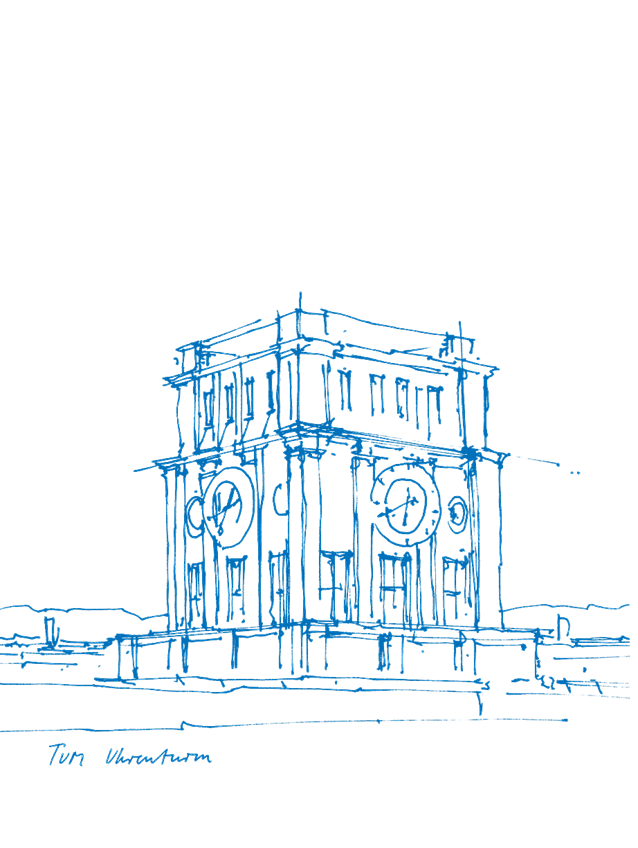
\includegraphics{./Ressourcen/Praesentation/Bilder/TUM_Uhrenturm.png}%
        \end{textblock*}
        \PraesentationTitelseiteInhalt
    }
}

\newcommand{\PraesentationStartseiteFlaggen}{
    \setbeamertemplate{title page}{%
        \begin{textblock*}{\paperwidth}[0,0](-\PraesentationSeitenrand,-\PraesentationSeitenrand)%
            \includegraphics[height=\paperheight]{./Ressourcen/Praesentation/Bilder/Universitaet_Flaggen.jpg}%
        \end{textblock*}
        \PraesentationSeitenkopfInhalt{./Ressourcen/_Bilder/Universitaet_Logo_weiss.pdf}
        \PraesentationTitelseiteInhalt
    }
}

\newcommand{\PraesentationStartseiteLeer}{
    \setbeamertemplate{title page}{%
        \PraesentationSeitenkopfInhalt{./Ressourcen/_Bilder/Universitaet_Logo_weiss.pdf}
        \PraesentationTitelseiteInhalt
    }
}


\newcommand{\PraesentationMasterStandard}{
    \PraesentationFarbschemaStandard

    \PraesentationStartseiteUhrenturm

    \setbeamertemplate{headline}{
        \PraesentationSeitenkopfInhalt{./Ressourcen/_Bilder/Universitaet_Logo_RGB.pdf}
    }
}

\newcommand{\PraesentationMasterWeissBlau}{
    \PraesentationFarbschemaWeissBlau

    \PraesentationStartseiteLeer

    \setbeamertemplate{headline}{
        \PraesentationSeitenkopfInhalt{./Ressourcen/_Bilder/Universitaet_Logo_weiss.pdf}
    }
}

\newcommand{\PraesentationMasterKopfzeileDreizeiler}{
    \PraesentationFarbschemaStandard

    \setbeamertemplate{title page}{%
        \begin{textblock*}{10.82cm}[0,1](0.9mm, \paperheight - 9mm)%
            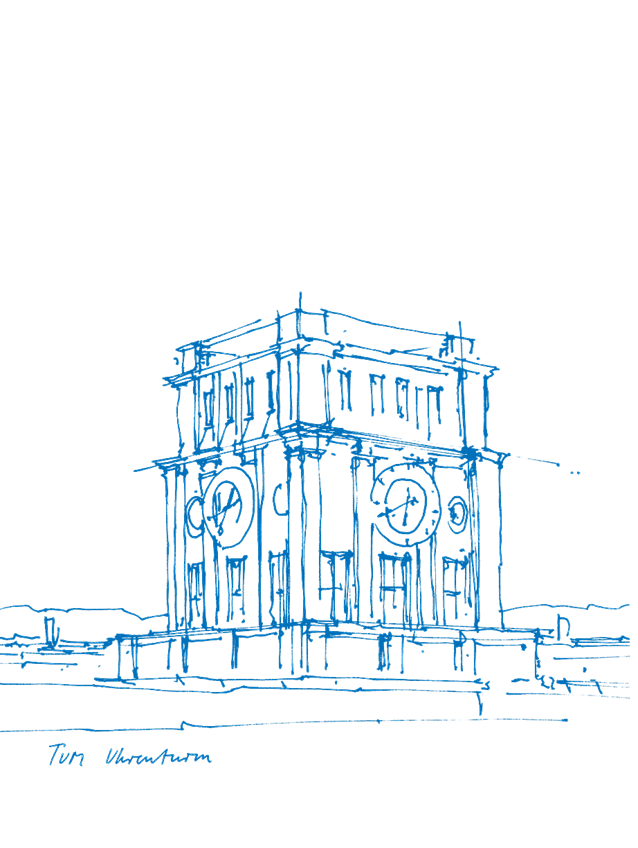
\includegraphics{./Ressourcen/Praesentation/Bilder/TUM_Uhrenturm.png}%
        \end{textblock*}
        \begin{textblock*}{\paperwidth}[0,0](0cm, -7.8mm)%
            \color{TUMBlau}\fontsize{7pt}{10pt}\selectfont%
            \LehrstuhlName\\%
            \FakultaetName\\%
            \UniversitaetName\\%
            \normalcolor\normalsize\selectfont%
        \end{textblock*}%
        \PraesentationSeitenkopfInhalt{./Ressourcen/_Bilder/Universitaet_Logo_RGB.pdf}
        \PraesentationTitelseiteInhalt
    }

    \setbeamertemplate{headline}{
        \begin{textblock*}{\paperwidth}[0,0](0cm, -7.8mm)%
            \color{TUMBlau}\fontsize{7pt}{10pt}\selectfont%
            \LehrstuhlName\\%
            \FakultaetName\\%
            \UniversitaetName\\%
            \normalcolor\normalsize\selectfont%
        \end{textblock*}%
        \PraesentationSeitenkopfInhalt{./Ressourcen/_Bilder/Universitaet_Logo_RGB.pdf}
    }
}

\newcommand{\PraesentationMasterWeissSchwarz}{
    \PraesentationFarbschemaWeissSchwarz

    \setbeamertemplate{title page}{%
        \PraesentationTitelseiteInhalt
        \PraesentationSeitenkopfInhalt{./Ressourcen/_Bilder/Universitaet_Logo_weiss.pdf}
    }

    \setbeamertemplate{headline}{
        \PraesentationSeitenkopfInhalt{./Ressourcen/_Bilder/Universitaet_Logo_weiss.pdf}
    }
}

\newcommand{\PraesentationTitelseite}{\frame[plain]{\titlepage}}
\newcommand{\PraesentationUeberschriftZweizeilig}[2]{\frametitle{#1\\[8mm]#2}}

\usepackage[
    orientation=portrait,
    size=custom,
    width=25.4,
    height=19.05,
    scale=0.63 % erzeugt 16pt Schriftgröße
]{beamerposter}
\setbeamersize{
    text margin left=\PraesentationSeitenrand,
    text margin right=\PraesentationSeitenrand
}

\setbeamerfont{framesubtitle}{size=\Large,series=\itshape}%

\setbeamertemplate{frametitle}{%
    {\rule{0pt}{31mm}\fontsize{31}{33}\selectfont\insertframetitle\newline\vspace*{-6.7mm}\\\usebeamerfont{framesubtitle}\insertframesubtitle}%
}

% Aufzählungen:
\newcommand{\PraesentationAufzaehlungEbeneEinsSymbol}{\raise2pt\hbox{\donotcoloroutermaths\usebeamercolor{itemize subitem}\fontsize{10pt}{8pt}$\bullet$}}
\newcommand{\PraesentationAufzaehlungEbeneZweiSymbol}{\raise1.25pt\hbox{\donotcoloroutermaths\usebeamercolor{itemize subitem}$-$}}
\setbeamertemplate{itemize items}[circle]
\setbeamertemplate{itemize subitem}[triangle]
\setbeamercolor{itemize subitem}{fg=black}
\setbeamerfont{itemize/enumerate subbody}{size=\normalsize}
\setbeamertemplate{itemize item}{\PraesentationAufzaehlungEbeneEinsSymbol}
\setbeamertemplate{itemize subitem}{\PraesentationAufzaehlungEbeneZweiSymbol{}}
%\addtolength{\leftmarginii}{16mm-2pt}%

\newenvironment{PraesentationAufzaehlung}
{%
    \vspace{-\baselineskip}%
    \begin{itemize}%
        \setlength{\itemsep}{0pt}%
        \setlength{\parskip}{0pt}%
        \setlength{\parsep}{0pt}%
        \addtolength{\itemindent}{-1ex}%
}{%
    \end{itemize}%
}

%%%%%%%%%%%%%%%%%%%%%%%%%%%%%%%%%%%%%%%%%%%%%%%%%%%%%%%%%%%%%%%%%%%%%%%%%%%%%%%%
% DOKUMENT
%%%%%%%%%%%%%%%%%%%%%%%%%%%%%%%%%%%%%%%%%%%%%%%%%%%%%%%%%%%%%%%%%%%%%%%%%%%%%%%%


% PDF-Einstellungen:
\hypersetup{
    pdfstartview={Fit},
    pdfproducer={\AllgemeinErsteller},
    pdfcreator={\AllgemeinGestalter}
}

\textblockorigin{\PraesentationSeitenrand}{\PraesentationSeitenrand} % Ursprung für Positionierung

\setbeamerfont{footnote}{size=\fontsize{12}{20}}

\setbeamertemplate{footline}{
    \hbox{%
        \usebeamerfont{footnote}%
        \begin{beamercolorbox}[wd=.9\paperwidth]{}%
            \hspace*{\PraesentationSeitenrand}%
            %\PersonTitel{} \PersonVorname~\PersonNachname~(\UniversitaetAbkuerzung) \PraesentationFusszeileZusatz{}%
             \PraesentationFusszeileZusatz{}%
        \end{beamercolorbox}%
        \begin{beamercolorbox}[wd=.1\paperwidth]{}%
        	\insertpagenumber{}%
            %\insertframenumber{}%
            \raggedleft
            \hspace*{\PraesentationSeitenrand}%
        \end{beamercolorbox}%
        \vspace*{3.25mm}%
    }%
}

\setbeamertemplate{navigation symbols}{}

\begin{document}
\setlength{\baselineskip}{22.1pt}
\setlength{\parskip}{\baselineskip}
 % !!! NICHT ENTFERNEN !!!
%%%%%%%%%%%%%%%%%%%%%%%%%%%%%%%%%%%%%%%%%%%%%%%%%%%%%%%%%%%%%%%%%%%%%%%%%%%%%%%%


%%%%%%%%%%%%%%%%%%%%%%%%%%%%%%%%%%%%%%%%%%%%%%%%%%%%%%%%%%%%%%%%%%%%%%%%%%%%%%%%
% FOLIENSTIL: Standard
%\PraesentationMasterStandard

%\PraesentationTitelseite % Fügt die Startseite ein

\lstset{
  language=XML,
  morekeywords={encoding,
    xs:schema,xs:element,xs:complexType,xs:sequence,xs:attribute},
  moredelim=**[is][\color{TUMBlauMittel}]{@}{@},
  moredelim=**[is][\color{TUMOrange}]{@@}{@@},
  moredelim=**[is][\color{TUMGruen}]{@@@}{@@@},
  moredelim=**[is][\color{gray!80}]{@@@@}{@@@@},
  showspaces=false,
  showstringspaces=false,
  breaklines=true,
  postbreak=\raisebox{0ex}[0ex][0ex]{\ensuremath{\color{gray}\hookrightarrow\space}},
}

%%%%%%%%%%%%%%%%%%%%%%%%%%%%%%%%%%%%%%%%%%%%%%%%%%%%%%%%%%%%%%%%%%%%%%%%%%%%%%%%
% FOLIENSTIL: Standard mit Lehrstuhl-, Fakultäts- und Universitätsnamen im
% Kopfbereich links
\PraesentationMasterKopfzeileDreizeiler

\PraesentationTitelseite

\PraesentationMasterStandard


\usetikzlibrary{shapes,arrows,shadows}
%%%%%%%%%%%%%%%%%%%%%%%%%%%%%%%%%%%%%%%%%%%%%%%%


%%%%%%%%%%%%%%%%%%%%%%%%%%%%%%%%%%%%%%

\begin{frame}[fragile]
	\frametitle{Agenda}
	\framesubtitle{}

	\textbf{Learning Goals}
	\begin{itemize}
		\item Become familiar with RIPE Atlas, its capabilities, and its use
		\begin{itemize}
			\item Who has used RIPE Atlas before?
		\end{itemize}
		\item See how to plan measurements and analyze data along the lines of a TMA'17 paper
		\item Run DNS and Traceroute measurements using RIPE Atlas
	\end{itemize}	

	\textbf{Outline}
\begin{itemize}
	\item Background on RIPE Atlas (previous lecture)
	\item Background on research questions to be answered
	\item DNS Measurements
	\item Traceroute Measurements
	\item Mapping to ASes/IXPs --- controversial discussion expected! \smiley{}
\end{itemize}	



\end{frame}
\clearpage

%%%%%%%%%%%%%%%%%%%%%%%%%%%%%%%%%%%%%%%%%%%%%%%%
\begin{frame}[fragile]
\frametitle{Background}

TMA'17 paper: \\
\textit{Push Away Your Privacy: Precise User Tracking Based on TLS Client Certificate Authentication}

\url{http://tma.ifip.org/wordpress/wp-content/uploads/2017/06/tma2017_paper2.pdf}

\end{frame}
\clearpage

%%%%%%%%%%%%%%%%%%%%%%%%%%%%%%%%%%%%%%

\begin{frame}[fragile]
\frametitle{Apple Push Notification Service (APNs)}
\framesubtitle{Maybe the biggest user of unencrypted TLS Client Certificate Authentication?}

\textbf{APNs integral part of iOS and macOS} -- ``always on''\\
%\begin{itemize}
%	\item ``Always on''
%	\item ``Cellular first''
%\end{itemize}

\textbf{APNs uses Client Certificates for login}:\\
\begin{itemize}
\item Generated at device setup
\item Unique cryptographic material (CN, public key, fingerprint)
\end{itemize}

\begin{verbatim}
Serial Number: ab:12:34:56:78:9a:bc:de:f0:12
Issuer: C=US, O=Apple Inc., OU=Apple iPhone, CN=Apple iPhone Device CA
Validity Not Before: Apr  8 12:34:56 2015 GMT
Validity Not After : Apr  8 12:34:56 2016 GMT
Subject: CN=12345678-1234-1234-1234-123456789ABC
Key ...
(all data redacted)
\end{verbatim}
\end{frame}
\clearpage

%%%%%%%%%%%%%%%%%%%%%%%%%%%%%%%%%%%%%%%%%%%%%%%%

\begin{frame}
\frametitle{Precise User Tracking in APNs}
\framesubtitle{Several appearances of same device easily linkable}

\textbf{2 attacker types}\\
\begin{itemize}
\item \st{Local adversary: Can use MAC addresses and more}
\item Regional adversary: Access to one or several large networks 
\item Global adversary: Access to several core networks
\end{itemize}

\textbf{Regional Adversary -- Feasibility Validation at Internet Uplink}\\
\begin{itemize}
%\item Respect User Privacy---Documented process, highly protected access \\
%$\rightarrow$ We were allowed to capture TLS CCA at MWN
\item Can a regional adversary track users?  \textbf{\textcolor{TUMGreen}{\checkmark}}
\end{itemize}

\textbf{Global Adversary -- Validation through Global Path Measurements}\\
\begin{itemize}
	\item How well can a global adversary leverage APNs to track users? \textcolor{red}{\textbf{This exercise}}
\end{itemize}

\end{frame}
\clearpage
%%%%%%%%%%%%%%%%%%%%%%%%%%%%%%%%%%%%%%%%%%%%%%%%
%%%%%%%%%%%%%%%%%%%%%%%%%%%%%%%%%%%%%%%%%%%%%%%%

\begin{frame}
\frametitle{Detailed Research Questions and Approach}
\framesubtitle{}

\textbf{Research Question: How many networks do you need to eavesdrop on to surveil a majority of APNs backend logins?}

Steps to be taken:
\begin{itemize}
	\item What and where are the APNs backend servers?
	\item How to measure paths for user population connecting to backend servers?
	\item How to map this to networks? What is a network in this context?
\end{itemize}

Take note: \textit{``Every paper has a flaw''} --- bonus points if you find them! \smiley{}

Questions?
\end{frame}
\clearpage
%%%%%%%%%%%%%%%%%%%%%%%%%%%%%%%%%%%%%%%%%%%%%%%%
%%%%%%%%%%%%%%%%%%%%%%%%%%%%%%%%%%%%%%%%%%%%%%%%

\begin{frame}
\frametitle{Step 1: Finding APNs Backend Servers}
\framesubtitle{}

From passive observations, we know that clients resolve [1-50]-courier.push.apple.com and then connect to 1 IP address in the 17.0.0.0/8 range.

How to find all APNs backend servers?
\pause

\textbf{Pick a country you want to work on! Inspiration: \url{http://sg-pub.ripe.net/petros/population_coverage/table.html}}
\pause

\textbf{Prerequisites}: \\ 
Do you have (a) RIPE Atlas Account (b) Voucher? (c) Python3 (d) Github Downloaded? \\
\texttt{git clone -{}-recursive git://github.com/quirins/tma17-ripeatlas-lab-participants}

\pause

\textbf{Task: Pick 1 of `[1-50]-courier.push.apple.com` and do a RIPE Atlas DNS resolution \\ for ``your'' country.}\\
Example: 42-courier.push.apple.com \\
New DNS measurement: \url{https://atlas.ripe.net/measurements/form/} \\
Note: More experienced RIPE Atlas users are invited to do resolutions for all 50 DNS names.

\end{frame}
\clearpage
%%%%%%%%%%%%%%%%%%%%%%%%%%%%%%%%%%%%%%%%%%%%%%%%
%%%%%%%%%%%%%%%%%%%%%%%%%%%%%%%%%%%%%%%%%%%%%%%%
\begin{frame}
\frametitle{Step 1: Finding APNs Backend Servers - Discussion}
\framesubtitle{}
\begin{itemize}
	\item What probes did you choose? How many per country? \hyperlink{NL example}{\url{http://sg-pub.ripe.net/petros/population_coverage/country.html?name=NL}}
	% XS4ALL example in NL: lots of probes, but not many users
	\item Which detailed DNS settings did you choose?
	\item How did you run the measurement? How to scale it to 50?
\end{itemize}
New DNS measurement: \url{https://atlas.ripe.net/measurements/form/} \\
Sample measurement from paper: \url{https://atlas.ripe.net/measurements/5500016/} \\
Sample measurement from June 2017: \url{https://atlas.ripe.net/measurements/8831682} \\
Script for batch measurements: \url{https://github.com/tumi8/cca-privacy/blob/master/ripe\_atlas/dns/atlas-measure.sh} \\

\end{frame}
\clearpage
%%%%%%%%%%%%%%%%%%%%%%%%%%%%%%%%%%%%%%%%%%%%%%%%
%%%%%%%%%%%%%%%%%%%%%%%%%%%%%%%%%%%%%%%%%%%%%%%%
\begin{frame}
\frametitle{Step 1: Finding APNs Backend Servers - Obtaining the Result}
\framesubtitle{}
\textbf{Your measurement should have finished by now -- please obtain the result and parse it} 

Our parsing script: \url{https://github.com/tumi8/cca-privacy/blob/master/ripe\_atlas/dns/parse-results.py}\\

\pause
 \textbf{Discussion}
 \vspace{-5mm}
\begin{itemize}
	\item Download via Browser or REST
	\item JSON with abuf
	\item Region-specific CNAMEs
	\item Are these all the IP addresses used by the APNs backend? Or just some?
\end{itemize}
\small{
Sample measurement result from June 2017: \url{https://github.com/quirins/tma17-ripeatlas-lab-participants/blob/master/data/dns/RIPE-Atlas-measurement-8831682.json}\\
Sample parsed result from paper \url{https://github.com/quirins/tma17-ripeatlas-lab-participants/blob/master/data/dns/result-5500014.json.parsed.txt} \\
Sample parsed result from June 2017 \url{https://github.com/quirins/tma17-ripeatlas-lab-participants/blob/master/data/dns/RIPE-Atlas-measurement-8831682.json.parsed.txt}\\
}

\end{frame}
\clearpage
%%%%%%%%%%%%%%%%%%%%%%%%%%%%%%%%%%%%%%%%%%%%%%%%

%%%%%%%%%%%%%%%%%%%%%%%%%%%%%%%%%%%%%%%%%%%%%%%%
\begin{frame}
\frametitle{Step 2: Traceroute Path Measurements}
\framesubtitle{}
Our DNS queries have yielded a list of backend servers. Coming back to our Research Question, we want to quantify the number of networks an adversary has to eavesdrop on to see a significant number of logins directed to those backend servers. \\
\textbf{Task: Define and execute a measurement strategy: Which RIPE Atlas settings? Which probes? Which targets?}\\
Note: Again, RIPE Atlas novices can just run 1 measurement towards 1 target IP address.

\pause
\textbf{Discussion}
\begin{itemize}
	\item Traceroute Details -- \url{https://atlas.ripe.net/measurements/form/}
	\item Target Selection -- all APNs IP addresses? Some? 
	\item Probe Selection:
	\begin{itemize}
		\item Which probes to select?
		\item Do they represent the APNs user base? AS/CC bias?
		\item Only probes that resolved the IP being probed?
	\end{itemize}
\end{itemize}

Traceroute measurement from Paper - Germany: \url{https://atlas.ripe.net/measurements/5719601/}
\end{frame}
\clearpage
%%%%%%%%%%%%%%%%%%%%%%%%%%%%%%%%%%%%%%%%%%%%%%%%
%%%%%%%%%%%%%%%%%%%%%%%%%%%%%%%%%%%%%%%%%%%%%%%%
\begin{frame}
\frametitle{Step 2: Traceroute Path Measurements}
\framesubtitle{}
\textbf{Task: Please download the results -- what format does it have? Ideas how to parse it? What would be the next steps?}
\pause
\begin{itemize}
	\item JSON -- RIPE Atlas Cousteau or raw JSON parsing
	\item Next step: Map to IXPs and ASes -- Ideas on data sources?
\end{itemize}
\pause
Fortunately, the link \url{https://github.com/tumi8/cca-privacy/tree/master/ripe_atlas/traceroute} contains the script ``traceroutes\_to\_asn\_ixp.py.''

\textbf{Task: Call it using ./traceroutes\_to\_asn\_ixp.py your-measurement.json ip2ixp ip2as}\\

ip2ixp (traiXroute/peeringDB): \url{https://github.com/tumi8/cca-privacy/blob/master/ripe_atlas/traceroute/ixp_subnets_v4.csv}
recent ip2as (CAIDA pfx2as): \url{http://data.caida.org/datasets/routing/routeviews-prefix2as/2017/06/routeviews-rv2-20170618-1000.pfx2as.gz}

Sample Result from Paper:\\ \url{https://github.com/quirins/tma17-ripeatlas-lab-participants/blob/master/data/traceroute/result-5719599.json.result.txt}

\end{frame}
\clearpage
%%%%%%%%%%%%%%%%%%%%%%%%%%%%%%%%%%%%%%%%%%%%%%%%
%%%%%%%%%%%%%%%%%%%%%%%%%%%%%%%%%%%%%%%%%%%%%%%%
\begin{frame}
\frametitle{Step 3: Analyze Results}
\framesubtitle{}

How does the result look like for your country? Is that in line with the paper?
\begin{table}[!h]%[b]
	\centering		
	%	\begin{minipage}{\textwidth}
	%\resizebox{\textwidth}{!}
	{\begin{tabular}{llrclr}
			\toprule
			Rank ~~~~~& \multicolumn{2}{c}{Global} && \multicolumn{2}{c}{Germany}	\\
			\cmidrule{2-3} \cmidrule{5-6}
			& IXP/AS  & \textSigma\% Paths &~~~& IXP/AS & \textSigma\% Paths   \\
			\midrule
			1 & AS3356 (L3)  & 25\%  && IXP DE-CIX & 30\% \\
			2 & AS1299 (Telia) & 40\%  && AS3320 (DTAG) & 52\% \\
			3 & AS174 (Cogent)  & 54\%  && IXP E-CIX & 61\% \\
			4 & AS7922 (Comcast)~~~  & 61\%  && AS6830 (Liberty) ~~~& 69\% \\
			5 & AS12322 (Free)  & 67\%  && AS31334 (VF/Kabel D) & 75\%\\
			6 & AS6830 (Liberty)  & 71\%  && AS1273 (C\&W)& 78\%\\
			7 & AS4637 (Telstra) & 75\%  && AS3356 (L3)  & 81\% \\
			8 & AS6453 (Tata) & 78\%  && AS34419 (VF Group)& 84\% \\
			9 & AS2828 (XO)  & 81\%  && AS680 (DFN) & 86\% \\
			10 & AS3320 (DTAG) & 84\% && AS6805 (Telefonica) & 88\% \\
			\bottomrule
	\end{tabular}}
\end{table}

\pause
\textbf{$\rightarrow$ What do you think of the result overall?}
\end{frame}
\clearpage

%%%%%%%%%%%%%%%%%%%%%%%%%%%%%%%%%%%%%%%%%%%%%%%%
%%%%%%%%%%%%%%%%%%%%%%%%%%%%%%%%%%%%%%%%%%%%%%%%
\begin{frame}
\frametitle{Feedback \& Conclusion}
\begin{itemize}
	\item How did you like the exercise?
	\item Useful parts / less useful parts?
	\item Excited to use RIPE Atlas? \smiley{}
\end{itemize}
\vspace{10mm}
\textbf{Black Belt Track}: Share your results back to the exercise through a pull-request. 

To do so, please use this folder structure:
\begin{itemize}
	\item tma17-ripeatlas-lab-participants/results/\$country/[dns|traceroute]
	\begin{itemize}
		\item A list of DNS and traceroute measurement IDs
		\item Intermediate Results (potentially compressed)
		\item the final table
		\item a readme file with: your name and a quick description of your approach
	\end{itemize}
\end{itemize}

\end{frame}
\clearpage


%%%%%%%%%%%%%%%%%%%%%%%%%%%%%%%%%%%%%%%%%%%%%%%%

\begin{frame}
\frametitle{Backup}
\end{frame}
\clearpage
%%%%%%%%%%%%%%%%%%%%%%%%%%%%%%%%%%%%%%%%%%%%%%%%


%%%%%%%%%%%%%%%%%%%%%%%%%%%%%%%%%%%%%%%%%%%%%%%%
\begin{frame}
	\frametitle{Is global tracking feasible?}
	\framesubtitle{Methodology}
	Research Question: How many networks does an attacker have to eavesdrop on to observe a significant share of APNs logins?
	\begin{itemize}
		\item We identify APNs backend infrastructure and conduct distributed traceroute \\ measurements towards it
		\begin{itemize}
		\item Measurements confirm that clients resolve one of \textit{[1-50]-courier.push.apple.com}
		\item We globally resolve \textit{[1-50]-courier.push.apple.com} using 1000 RIPE Atlas probes each
		\item We find 69 /24 subnets and pick one random observed IP address in each of the 69 subnets
		\item Using 1000 RIPE Atlas probes per measurement, we conduct traceroute measurements towards all 69 IP addresses
		\end{itemize}
		\item We map transit router's IP addresses to ISPs and IXPs
		\item We count what \% of routes traverses a certain ISP or IXP
	\end{itemize}	
\end{frame}
%%%%%%%%%%%%%%%%%%%%%%%%%%%%%%%%%%%%%%%%%%%%%%%%
%%%%%%%%%%%%%%%%%%%%%%%%%%%%%%%%%%%%%%%%%%%%%%%%
%%%%%%%%%%%%%%%%%%%%%%%%%%%%%%%%%%%%%%%%%%%%%%%%%%%%%%%%%%%%%%%%%%%%%%%%%%%%%%%%
% FOLIENSTIL: Weisse Schrift auf blauem Grund
%\PraesentationMasterWeissBlau

%%%%%%%%%%%%%%%%%%%%%%%%%%%%%%%%%%%%%%%%%%%%%%%%%%%%%
%% Startseiten                                     %%

% Setzt die Startseite auf eine mit Flaggen als Hintergrund:
%\PraesentationStartseiteFlaggen

% Setzt die Startseite auf eine mit mit einer Zeichnung des TUM-Uhrenturms:
%\PraesentationStartseiteUhrenturm

% Setzt die Startseite auf eine ohne Hintergrund:
%\PraesentationStartseiteLeer

%\PraesentationTitelseite % Fügt die Startseite ein
%%%%%%%%%%%%%%%%%%%%%%%%%%%%%%%%%%%%%%%%%%%%%%%%%%%%%


%\begin{frame}
%    \PraesentationUeberschriftZweizeilig{Präsentationsmuster}{%
%        kann auch als Kapiteltrenner verwendet werden}
%\end{frame}

%%%%%%%%%%%%%%%%%%%%%%%%%%%%%%%%%%%%%%%%%%%%%%%%%%%%%%%%%%%%%%%%%%%%%%%%%%%%%%%%
% FOLIENSTIL: Weisse Schrift auf schwarzem Grund
%\PraesentationMasterWeissSchwarz

%%%%%%%%%%%%%%%%%%%%%%%%%%%%%%%%%%%%%%%%%%%%%%%%%%%%%%%%%%%%%%%%%%%%%%%%%%%%%%%%
\end{document} % !!! NICHT ENTFERNEN !!!
%%%%%%%%%%%%%%%%%%%%%%%%%%%%%%%%%%%%%%%%%%%%%%%%%%%%%%%%%%%%%%%%%%%%%%%%%%%%%%%%
